% -----------------------------------------------
% Template for ISMIR Papers
% 2020 version, based on previous ISMIR templates

% Requirements :
% * 6+n page length maximum
% * 4MB maximum file size
% * Copyright note must appear in the bottom left corner of first page
% * Clearer statement about citing own work in anonymized submission
% (see conference website for additional details)
% -----------------------------------------------

\documentclass{article}
\usepackage[T1]{fontenc} % add special characters (e.g., umlaute)
\usepackage[utf8]{inputenc} % set utf-8 as default input encoding
\usepackage{ismir,amsmath,cite,url}
\usepackage{graphicx}
\usepackage{color}

% Optional: To use hyperref, uncomment the following.
% \usepackage[bookmarks=false,hidelinks]{hyperref}
% Mind the bookmarks=false option; bookmarks are incompatible with ismir.sty.

\usepackage{lineno}
\linenumbers

% Title.
% ------
\title{Paper Template For ISMIR \conferenceyear}

% Note: Please do NOT use \thanks or a \footnote in any of the author markup

% Single address
% To use with only one author or several with the same address
% ---------------
%\oneauthor
% {Names should be omitted for double-blind reviewing}
% {Affiliations should be omitted for double-blind reviewing}

% Two addresses
% --------------
%\twoauthors
%  {First author} {School \\ Department}
%  {Second author} {Company \\ Address}

%% To make customize author list in Creative Common license, uncomment and customize the next line
%  \def\authorname{First Author, Second Author}


% Three addresses
% --------------
\threeauthors
  {First Author} {Affiliation1 \\ {\tt author1@ismir.edu}}
  {Second Author} {\bf Retain these fake authors in\\\bf submission to preserve the formatting}
  {Third Author} {Affiliation3 \\ {\tt author3@ismir.edu}}

%% To make customize author list in Creative Common license, uncomment and customize the next line
%  \def\authorname{First Author, Second Author, Third Author}

% Four or more addresses
% OR alternative format for large number of co-authors
% ------------
%\multauthor
%{First author$^1$ \hspace{1cm} Second author$^1$ \hspace{1cm} Third author$^2$} { \bfseries{Fourth author$^3$ \hspace{1cm} Fifth author$^2$ \hspace{1cm} Sixth author$^1$}\\
%  $^1$ Department of Computer Science, University , Country\\
%$^2$ International Laboratories, City, Country\\
%$^3$  Company, Address\\
%{\tt\small CorrespondenceAuthor@ismir.edu, PossibleOtherAuthor@ismir.edu}
%}
%\def\authorname{First author, Second author, Third author, Fourth author, Fifth author, Sixth author}


\sloppy % please retain sloppy command for improved formatting

\begin{document}

%
\maketitle
%
\begin{abstract}
The abstract should be placed at the top left column and should contain about 150-200 words.
\end{abstract}
%
\section{Introduction}\label{sec:introduction}

This template includes all the information about formatting manuscripts for the ISMIR \conferenceyear\ Conference.
Please follow these guidelines to give the final proceedings a uniform look.
Most of the required formatting is achieved automatically by using the supplied
style file (\LaTeX) or template (Word).
If you have any questions, please contact the Program Committee (\texttt{ismir\conferenceyear-papers@ismir.net}).
This template can be downloaded from the ISMIR \conferenceyear\ web site (\texttt{http://ismir\conferenceyear.ismir.net}).
%
\section{Paper Length \& File Size}
We adopt a ``(6+n)-page policy'' for ISMIR \conferenceyear. That is, each paper may have a maximum of six pages of technical content (including figures and tables) \textcolor{red}{with additional optional pages that contain only references and acknowledgments. Note that acknowledgments should not be included in the anonymized submission.}

Paper should be submitted as PDFs and the \textcolor{red}{file size is limited to 4MB}. Please compress images and figures as necessary before submitting.

\section{Page Size}\label{sec:page_size}

The proceedings will be printed on
 \underline{portrait A4-size paper} \underline{(21.0cm x 29.7cm)}.
All material on each page should fit within a rectangle of 17.2cm x 25.2cm,
centered on the page, beginning 2.0cm
from the top of the page and ending with 2.5cm from the bottom.
The left and right margins should be 1.9cm.
The text should be in two 8.2cm columns with a 0.8cm gutter.
All text must be in a two-column format.
Text must be fully justified.

\section{Typeset Text}\label{sec:typeset_text}

\subsection{Normal or Body Text}\label{subsec:body}

Please use a 10pt (point) Times font. Sans-serif or non-proportional fonts
can be used only for special purposes, such as distinguishing source code text.

The first paragraph in each section should not be indented, but all other paragraphs should be.

\subsection{Title and Authors}

The title is 14pt Times, bold, caps, upper case, centered.
\textcolor{red}{Authors' names are omitted when submitting for double-blind reviewing.}
The following is for making a camera-ready version.
Authors' names are centered.
The lead author's name is to be listed first (left-most), and the co-authors' names after.
If the addresses for all authors are the same, include the address only once, centered.
If the authors have different addresses, put the addresses, evenly spaced, under each authors' name.

\subsection{First Page Copyright Notice}

Please include the copyright notice exactly as it appears here in the lower left-hand corner of the page.
It is set in 8pt Times. \textcolor{red}{After your paper is accepted, you will need to insert the appropriate author names and paper title in the copyright notice when submitting the camera-ready version.} For \LaTeX users, this will be handled by the template automatically. For Word users, this has to be done manually.


\subsection{Page Numbering, Headers and Footers}

Do not include headers, footers or page numbers in your submission.
These will be added when the publications are assembled.

\subsection{Line Numbers}

Line numbers should be included in your originally submitted manuscript, for reference during reviewing. \textcolor{red}{However, after your paper is accepted, you must remove all line numbers from the final camera-ready version.} This can be done in \LaTeX by commenting out the command \verb|\linenumbers| on Line 25. This can be done in Microsoft Word by selecting Layout > Line Numbers > None.

\section{First Level Headings}

First level headings are in Times 10pt bold,
centered with 1 line of space above the section head, and 1/2 space below it.
For a section header immediately followed by a subsection header, the space should be merged.

\subsection{Second Level Headings}

Second level headings are in Times 10pt bold, flush left,
with 1 line of space above the section head, and 1/2 space below it.
The first letter of each significant word is capitalized.

\subsubsection{Third and Further Level Headings}

Third level headings are in Times 10pt italic, flush left,
with 1/2 line of space above the section head, and 1/2 space below it.
The first letter of each significant word is capitalized.

Using more than three levels of headings is highly discouraged.

\section{Footnotes and Figures}

\subsection{Footnotes}

Indicate footnotes with a number in the text.\footnote{This is a footnote.}
Use 8pt type for footnotes. Place the footnotes at the bottom of the page on which they appear.
Precede the footnote with a 0.5pt horizontal rule.

\subsection{Figures, Tables and Captions}

All artwork must be centered, neat, clean, and legible.
All lines should be very dark for purposes of reproduction and art work should not be hand-drawn.
The proceedings are not in color, and therefore all figures must make sense in black-and-white form.
Figure and table numbers and captions always appear below the figure.
Leave 1 line space between the figure or table and the caption.
Each figure or table is numbered consecutively. Captions should be Times 10pt.
Place tables/figures in text as close to the reference as possible.
References to tables and figures should be capitalized, for example:
see \figref{fig:example} and \tabref{tab:example}.
Figures and tables may extend across both columns to a maximum width of 17.2cm.

\begin{table}
 \begin{center}
 \begin{tabular}{|l|l|}
  \hline
  String value & Numeric value \\
  \hline
  Hello ISMIR  & \conferenceyear \\
  \hline
 \end{tabular}
\end{center}
 \caption{Table captions should be placed below the table.}
 \label{tab:example}
\end{table}

\begin{figure}
 \centerline{\framebox{
 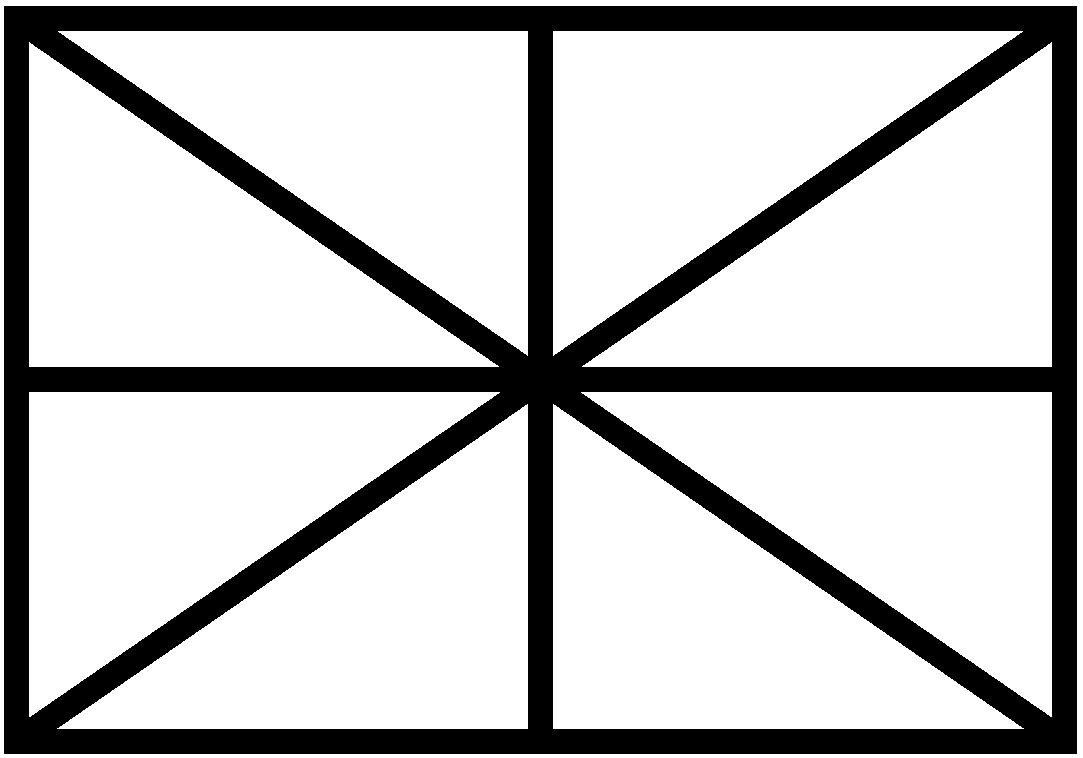
\includegraphics[width=\columnwidth]{figure.png}}}
 \caption{Figure captions should be placed below the figure.}
 \label{fig:example}
\end{figure}

\section{Equations}

Equations should be placed on separate lines and numbered.
The number should be on the right side, in parentheses, as in \eqnref{relativity}.

\begin{equation}\label{relativity}
E=mc^{2}
\end{equation}

\section{Citations}

All bibliographical references should be listed at the end,
inside a section named ``REFERENCES,'' numbered and in alphabetical order.
All references listed should be cited in the text.
When referring to a document, type the number in square brackets
\cite{Author:00}, or for a range \cite{Author:00,Someone:10,Someone:04}.

When the following words appear in the conference publication titles, please abbreviate them: Proceedings $\rightarrow$ Proc.; Record $\rightarrow$ Rec.; Symposium $\rightarrow$ Symp.; Technical Digest $\rightarrow$ Tech. Dig.; Technical Paper $\rightarrow$ Tech. Paper; First $\rightarrow$ 1st; Second $\rightarrow$ 2nd; Third $\rightarrow$ 3rd; Fourth/nth $\rightarrow$ 4th/nth.

\textcolor{red}{As submission is double blind, refer to your own published work in the third person. That is, use ``In the previous work of \cite{Someone:10},'' not ``In our previous work \cite{Someone:10}.'' If you cite your other papers that are not widely available (e.g., a journal paper under review), use anonymous author names in the citation, e.g., an author of the form ``A. Anonymous.''}

% For bibtex users:
\bibliography{ISMIRtemplate}

% For non bibtex users:
%\begin{thebibliography}{citations}
%
%\bibitem {Author:00}
%E. Author.
%``The Title of the Conference Paper,''
%{\it Proceedings of the International Symposium
%on Music Information Retrieval}, pp.~000--111, 2000.
%
%\bibitem{Someone:10}
%A. Someone, B. Someone, and C. Someone.
%``The Title of the Journal Paper,''
%{\it Journal of New Music Research},
%Vol.~A, No.~B, pp.~111--222, 2010.
%
%\bibitem{Someone:04} X. Someone and Y. Someone. {\it Title of the Book},
%    Editorial Acme, Porto, 2012.
%
%\end{thebibliography}

\end{document}

